\chapter{Evaluation}

\section{Evaluation Methodology}
Evaluating a real-time continuity monitoring system requires balancing traditional computer vision metrics with production-specific constraints. Unlike conventional object detection benchmarks that prioritise accuracy alone, film production demands both precision and speed. This evaluation therefore examines three main properties: detection accuracy to ensure reliability, processing speed to enable real-time operation and practical applicability within production workflows.

\subsection{Evaluation Metrics}
\textbf{mAP (mean Average Precision)}: Following standard object detection evaluation practices, we adopt mAP as our primary accuracy metric for DifferenceDetector. Modern detection systems including YOLOv11 [16] and Detectron2 [18] utilise mAP at various IoU thresholds to comprehensively assess detection quality.

\textbf{Accuracy}: ClockDetector in its nature solves classification problem, so even though it utilises YOLOv11 for object detection, the overall performance can be summarised using accuracy, precision, recall and F1.

\textbf{Time to Detection (TtD)}: End-to-end processing time from frame capture to result, ensuring detection completes within production reset windows.

\textbf{False Positive/Negative Rates}: Separate error analysis since missed continuity errors cost significantly more than false alerts in post-production.

\subsection{Test Environment}
We deliberately chose consumer-grade hardware for evaluation to reflect realistic deployment scenarios:
\begin{itemize}
\item CPU: Intel Core i9-11900 (8 cores, 5.3GHz boost)
\item GPU: NVIDIA RTX 3050 (4GB VRAM, GPU acceleration enabled)
\item RAM: 32GB DDR4-3200
\item Storage: 1TB NVMe SSD
\item Total cost: approximately £2,000
\end{itemize}

\subsection{Dataset Composition}
The selection of evaluation datasets presented unique challenges, as no existing benchmarks specifically address film continuity detection. To properly evaluate the overall performance we use tailored datasets for each detector. Table 5.1 summarises the dataset characteristics and their evaluation purposes.

\begin{table}[h]
\centering
\caption{Dataset Composition for both ClockDetector and DifferenceDetector}
\label{tab:datasets}
\begin{tabular}{llll}
\toprule
\textbf{Dataset} & \textbf{Type} & \textbf{Size} & \textbf{Purpose} \\
\midrule
\multicolumn{4}{l}{\textit{ClockDetector Datasets}} \\
ClockMovies & Real film footage & 1,131 images & Analogue clock variety \\
Synthetic digital & Generated & 100 images & Digital clock precision \\
\midrule
\multicolumn{4}{l}{\textit{DifferenceDetector Datasets}} \\
COCO-Inpainted (small) & Modified photos & 1,655 pairs & Small object changes (<32² px) \\
COCO-Inpainted (medium) & Modified photos & 1,747 pairs & Medium objects (32²-96² px) \\
COCO-Inpainted (large) & Modified photos & 1,006 pairs & Large objects (>96² px) \\
SynthText-Change & Synthetic & 5,000 pairs & Text modifications \\
VIRAT-STD & Surveillance & 26,155 pairs & Outdoor scenes \\
Kubric-Change & 3D rendered & 1,604 pairs & Geometric transformations \\
\bottomrule
\end{tabular}
\end{table}

\section{Performance Analysis}

\subsection{ClockDetector}
ClockDetector demonstrated robust classification performance across 1,231 test images from film footage and synthetic clocks. The detector overall achieved:
\begin{itemize}
\item Accuracy: 75.0\% (923/1231 correct classifications)
\item Precision: 81.4\% (923/1134 true positives among detections)
\item Recall: 75.0\% (923/1231 clocks correctly identified and read)
\item F1 Score: 0.78
\end{itemize}

These metrics reveal balanced performance between precision and recall, with the system correctly reading time in 81.4\% of detected clocks whilst identifying 75\% of all clocks in the dataset. Digital and analog clocks showed distinct performance characteristics (Table 5.2):

\begin{table}[h]
\centering
\caption{ClockDetector Performance for each clock type}
\label{tab:clock-performance}
\begin{tabular}{llllll}
\toprule
\textbf{Clock Type} & \textbf{Total} & \textbf{Correct} & \textbf{Accuracy} & \textbf{Precision} & \textbf{Recall} \\
\midrule
Analog & 1,131 & 832 & 73.6\% & 80.3\% & 89.8\% \\
Digital & 100 & 91 & 91.0\% & 92.9\% & 97.8\% \\
\bottomrule
\end{tabular}
\end{table}

Digital clock recognition performed well at a high 91\% accuracy through PaddleOCR's text detection capabilities. However, the limited test set of 100 images indicates a need for more thorough evaluation on larger datasets to validate this performance across diverse digital display types and more complex scene setups.

Analog clocks proved more challenging at 73.6\% accuracy. While this falls below Yang et al.'s reported ~80\% [23], our precision of 80.3\% aligns more closely with their findings. This discrepancy likely stems from our addition of YOLOv11 as a detection layer before time reading, which introduces an extra failure point where clocks might not be detected at all, thus reducing overall accuracy whilst maintaining high precision on detected clocks. The systematic challenges for analog clock recognition included:
\begin{itemize}
\item Extreme viewing angles where STN homography failed to normalise the clock face
\item Decorative faces lacking clear hour markers, common in period films
\item Low-contrast scenes typical in film noir where clock hands blend with backgrounds
\end{itemize}

Time to Detection averaged 1.92 seconds per frame pair, with the majority of processing time (83.1\%) consumed by the time reading. Either the STN and ResNet50 pipeline for analog clocks or PaddleOCR scanning for digital displays. 

The error distribution reveals that most errors occurred during time reading rather than detection. YOLOv11 successfully identifies clocks in 92.1\% of images. 
\begin{itemize}
\item False Negatives (No detection): 97 images where no clock was found
\item False Positives (Incorrect reading): 211 images where clocks were detected but time was misread
\end{itemize}

As previously discussed we aim for low miss rates (false negatives), since it leads to costly post production fixes. Evaluation revealed that ClockDetector outperforms in this metric with just 7.9\% failures.

\subsection{DifferenceDetector}
DifferenceDetector achieved 60.7\% mean Average Precision (mAP) at IoU 0.5 across 38,167 test frame pairs, almost matching the baseline performance reported by Sachdeva and Zisserman [22]. This demonstrates successful adaptation of their co-attention architecture to film production contexts, despite our additional masking and filtering stages. We can see detector's strength and limitations from its performance on different datasets (Table 5.3):

\begin{table}[h]
\centering
\caption{DifferenceDetector performance across evaluation datasets}
\label{tab:difference-performance}
\begin{tabular}{llll}
\toprule
\textbf{Dataset} & \textbf{mAP} & \textbf{Key Characteristics} & \textbf{Frames} \\
\midrule
COCO small & 0.462 & Challenging small objects & 1,655 \\
COCO medium & 0.787 & Optimal detection range & 1,747 \\
COCO large & 0.850 & Easiest size category & 1,006 \\
COCO combined & 0.627 & - & 4,408 \\
SynthText-Change & 0.890 & High contrast text & 5,000 \\
VIRAT-STD & 0.540 & Outdoor lighting variations & 26,155 \\
Kubric-Change & 0.761 & 3D transformations & 1,604 \\
\bottomrule
\end{tabular}
\end{table}

Performance correlates strongly with object size, dropping from 85\% for large changes to 46.2\% for small objects. Outdoor surveillance footage with dynamic lighting conditions poses significant challenges for the detector, along with other kinds of occlusions and fine detail. The consistent performance across synthetic and real-world datasets suggests reasonable generalisation to production footage.

Time to Detection averaged 6.37 seconds per frame pair, substantially longer than ClockDetector. This processing time reflects the computational complexity of co-attention mechanisms operating at multiple feature scales.

\subsection{Detection Accuracy}
The evaluation results reveal a critical distinction between achieving technical benchmarks and production viability. In Section 3.1.2, we established human script supervisor accuracy at 75-80\% over 10-14 hour production days, based on vigilance task research [9]. Against this baseline, ClockDetector's 75\% accuracy technically meets human performance levels, suggesting reliable deployment potential for temporal continuity monitoring.

However, DifferenceDetector's 60.7\% mAP falls substantially short of human capability. This 15-20\% performance gap becomes more pronounced considering the detector's sensitivity to environmental conditions. Outdoor scenes achieved only 54\% mAP versus 89\% on high-contrast synthetic data. Such variance indicates unreliable performance across diverse production environments, from controlled studio sets to dynamic location shoots.

These results definitively position CAM-F as an assistive rather than autonomous system. ClockDetector can reliably flag temporal inconsistencies for supervisor verification, while DifferenceDetector serves best as a preliminary filter for obvious spatial changes.

\subsection{Real-time Viability}
Determining real-time performance requires more nuance than simple frame rates. We developed a custom metric that calculates the maximum capture frame rate sustainable within production constraints, accounting for processing backlogs during takes and recovery during reset windows. We introduce a Production-Aligned Frame Rate (PAFR) metric that calculates the maximum capture rate sustainable during filming whilst guaranteeing all processing completes before the next take begins.

Given:
\begin{itemize}
\item x = time-to-detect per frame pair (seconds)
\item y = capture frame rate (fps)
\item S = typical take duration (seconds)
\item R = reset window between takes (seconds)
\end{itemize}

The system operates in one of two modes:

\textbf{Strict real-time}: Processing keeps pace with capture, requiring:
$$y \leq \frac{1}{x}$$

\textbf{Production real-time}: Frames queue during filming but clear during reset. The queue grows at $(y - \frac{1}{x})$ fps during the S-second take, creating a backlog:
$$q(S) = \left(y - \frac{1}{x}\right) \cdot S$$

These frames require time to process:
$$T_{\text{clear}} = S \cdot (y \cdot x - 1)$$

To finish before the next take, we need $T_{\text{clear}} \leq R$, yielding maximum sustainable frame rate:
$$y_{\text{max}} = \frac{\frac{R}{S} + 1}{x}$$

As we previously discussed in the system requirements, workflows and timings differ significantly depending on the size of the production. For the sake of grounding the system and evaluating its temporal performance we assume the most common scenario, where each take is about 45 seconds, while reset time is 5 minutes. In such case:

\textbf{ClockDetector Analysis}

With x = 1.92s per frame pair:
\begin{itemize}
\item Strict real-time: $y \leq \frac{1}{1.92} = 0.52$ fps
\item Production real-time (45s take, 300s reset):
$$y_{\text{max}} = \frac{\frac{300}{45} + 1}{1.92} = \frac{7.67}{1.92} = 4.0 \text{ fps}$$
\end{itemize}

With the PAFR of 4fps, ClockDetector would capture every 6th frame of the 24fps incoming feed.

\textbf{DifferenceDetector Analysis}

With x = 6.37s per frame pair:
\begin{itemize}
\item Strict real-time: $y \leq \frac{1}{6.37} = 0.16$ fps
\item Production real-time (45s take, 300s reset):
$$y_{\text{max}} = \frac{\frac{300}{45} + 1}{6.37} = \frac{7.67}{6.37} = 1.2 \text{ fps}$$
\end{itemize}

With the PAFR of 1.2fps, DifferenceDetector would capture approximately every 20th frame of the 24fps incoming feed.

\begin{figure}[h]
\centering
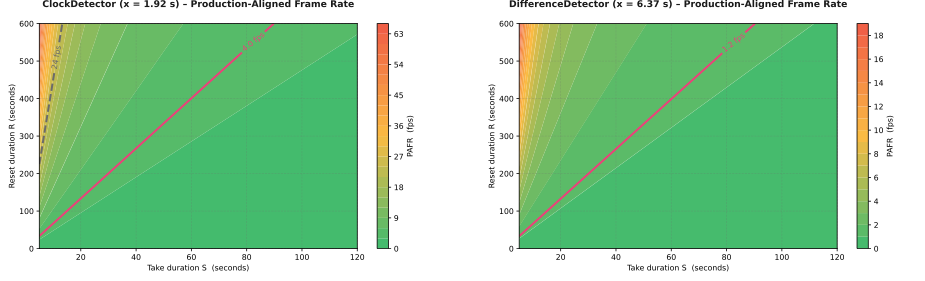
\includegraphics[width=\textwidth]{figures/PAFRplot.png}
\caption{Production-Aligned Frame Rate (PAFR) analysis showing the relationship between capture frame rate and backlog clearing time for both detectors. The intersection of each detector curve with the 300-second reset window (red dashed line) determines maximum sustainable frame rates: 4.0 fps for ClockDetector and 1.2 fps for DifferenceDetector. The shaded region indicates frame rates that would cause production delays by exceeding available reset time. System-wide performance is constrained by the slowest detector at 1.2 fps.}
\label{fig:pafr}
\end{figure}

When running multiple detectors concurrently, the system must synchronise frame distribution to maintain consistency. The slowest detector constrains the entire pipeline to 1.2fps in our case. This infrequent sampling proves sufficient as continuity errors typically persist for some time. The PAFR metric aims to confine CAM-F within its limitations and ensure that processing backlogs never exceed reset windows, guaranteeing detection results arrive before the next take begins without production delays. Figure 5.1 visualises these PAFR calculations across different production scenarios.

\subsection{Workflow Integration Testing}
Integration testing evaluated CAM-F under simulated production conditions using staged scenes with 12 planted continuity errors. Testing consisted of static takes from multiple angles and motion sequences with both actor and camera movement. Each scene employed carefully tuned detector configurations, which are available in the UI, demonstrating the importance of scene-specific parameter adjustment for optimal performance.

\textbf{Test Configuration and Results}

The system processed approximately 30 seconds of footage at 1 FPS capture rate, completing detection within 3 minutes post-take. This performance aligns with our PAFR metric calculations, which allows up to 1.1 FPS for this take-reset configuration to maintain production workflow compatibility. The interface successfully displayed real-time detection results and we managed to generate structured reports without any disruptions.

CAM-F detected 10 out of 12 planted errors (83.3\% recall) with 71-77\% precision. Static scenes detected 7/9 errors (77.8\%) with 3-4 false positives (see Figures 5.2 and 4.5), while motion scenes achieved perfect detection (3/3) with zero false positives (see Figure 5.3). This performance exceeds the dataset evaluation results, where DifferenceDetector achieved only 60.7\% mAP. The improved accuracy partly comes from the limited test cases, but more significantly from the fundamental difference in image quality. Benchmark datasets contain images of highly variable quality: compressed web images, surveillance footage and amateur photography. Professional film production maintains consistent high resolution and visual clarity. Modern cameras can capture at 4K or even higher with proper lighting and focus. This quality consistency gives detection algorithms cleaner features to analyse and improves object detection. Our results suggest that CAM-F may perform more reliably in actual production environments than synthetic benchmarks predict, as professional footage provides optimal conditions for computer vision algorithms.

\begin{figure}[h]
\centering
\includegraphics[width=\textwidth]{figures/statictest.png}
\caption{Integration test results from static scene. Wide-angle shot captured over 30 seconds at 1 fps, showing frame 30 with detection overlay.}
\label{fig:static-shots}
\end{figure}

The motion scene's perfect detection rate requires important clarification. We achieved 3/3 error detection using 2 FPS capture over 15 seconds (see Figure 5.3), which would exceed acceptable PAFR. Initial testing at the standard 1 FPS rate missed one of the errors. A book at the frame edge during camera movement appeared only briefly between sampled frames. The error became detectable only when we doubled the capture rate to 2 FPS. This shows a fundamental limitation of PAFR-constrained processing. Motion-heavy takes are much more likely to have temporal windows where errors exist for mere fractions of a second. At 1 FPS, the system samples every 24th frame, creating about 0.96-second blind spots where such errors escape detection entirely. CAM-F's effectiveness, in its current computational capabilities, diminishes proportionally with scene's dynamics, making it most suitable for dialogue scenes and static setups rather than action sequences.

\begin{figure}[h]
\centering
\includegraphics[width=\textwidth]{figures/motiontest.png}
\caption{Integration test results from dynamic scene with camera movement. 15-second sequence captured at 2 fps, showing frames 6 and 26. Detection performance remained consistent despite motion, though higher capture rate was required to detect transient errors.}
\label{fig:dynamic-shots}
\end{figure}

The UI effectively supported the complete workflow from capture to documentation. Detection results appeared immediately in the error log with clear frame references and confidence scores. The false positive flagging interface allowed us to mark those incorrect detections we got in the experiment, removing them from the active error list. The PDF export contains all the findings and we could also add extra notes for clarity. This end-to-end workflow successfully imitated actual production practices where script supervisors quickly verify, annotate, and distribute continuity information. The system's ability to generate structured documentation within minutes of take completion shows us potential in its practical readiness for set deployment.

\begin{figure}[h]
\centering
\includegraphics[width=\textwidth]{figures/app.png}
\caption{CAM-F workflow interface showing real-time monitoring dashboard, detection results and generated PDF continuity report.}
\label{fig:app-interface}
\end{figure}

\section{Discussion}

\subsection{Results Overview}
The evaluation demonstrates that CAM-F achieves partial fulfilment of its design objectives. The system successfully implements real-time continuity monitoring within production constraints, processing all captured frames before subsequent takes commence. However, performance metrics reveal significant variance between detector implementations, with ClockDetector achieving human-equivalent accuracy and DifferenceDetector operating substantially below production needs, though integration testing revealed more promising results.

ClockDetector's 75\% accuracy aligns with the human performance baseline of 75-80\%, that we established based on study by Warm et al. [9] for sustained vigilance tasks, suggesting viable deployment potential for temporal continuity monitoring. The detector's 80.3\% precision on detected analog clocks demonstrates reliable performance when objects are successfully identified. Digital clock recognition also performed exceptionally well at 91\% accuracy through PaddleOCR, though it can be explained with a limited test set.

DifferenceDetector's 60.7\% mAP falls 15-20\% below human capability, rendering it suitable only as a preliminary filter rather than autonomous detection. Performance variance across datasets, from 89\% on high-contrast synthetic data to 54\% on outdoor surveillance footage, indicates environmental sensitivity that might be problematic across diverse production settings. However, integration testing production-quality footage achieved 83.3\% overall recall, suggesting that real environments on-set with consistent high-resolution capture may yield substantially better performance than synthetic benchmarks indicate. Nevertheless, the detector successfully adapts Sachdeva and Zisserman's co-attention architecture [22] to production contexts, demonstrating feasibility even if practical limitations remain.

The Production-Aligned Frame Rate metric reveals system-wide performance constrained to 1.2fps by DifferenceDetector's 6.37-second processing time. Whilst this appears restrictive compared to standard 24fps capture, Schmidt et al. [25] demonstrated that sampling films at one frame per second provides sufficient temporal resolution for narrative analysis, as consecutive frames share approximately 90\% similarity.

\subsection{Limitation Analysis}
\textbf{Error Coverage}: The current implementation partially addresses only two of the four major continuity error categories identified in Table 2.1. ClockDetector monitors temporal continuity through time-display analysis, while DifferenceDetector identifies spatial continuity violations through object displacement. However, action continuity and technical continuity remain entirely unaddressed. Combined, proposed detectors handle about 15\% of various continuity anomalies.

\textbf{FPS Constraints}: The 1.2 fps sampling rate, constrained by DifferenceDetector's processing time, introduces temporal blind spots in continuity monitoring. At this rate, the system captures approximately every 20th frame from standard 24fps footage, creating 0.79-second gaps between analysed frames. Critical limitations emerge in high-motion scenarios where camera movement or rapid set changes could cause errors to appear and disappear between sampled frames.

\textbf{Frame Alignment}: The absence of temporal synchronisation between reference and current takes creates systematic comparison errors. Takes rarely begin at precisely the same narrative moment due to the manual nature of capture controls. Spacial alignment is another issue that may arise through accidental camera adjustments or specific creative decisions. Since both implemented detectors are agnostic to temporal and spatial misalignment we prioritised other features over this one. However, in a reliable system with high monitoring standards, it is an essential preprocessing step.

\textbf{Dataset Validity}: The evaluation relies entirely on synthetic and modified datasets rather than authentic film footage. Since none of it is available in public access, we're left to use detector specific compositions. COCO-Inpainted image and other datasets we used lack the visual and functional characteristics of real film production.